%%%%%%%%%%%%%%%%%%%%%%%%%%%%%%%%%%%%%%%%%%%%%%%%%%%%%%%%%%%%%%%%%%%%%%%%%%%%%
\section{Hybrid MPI+Threads Programming}\label{sec:back-hybrid}
%%%%%%%%%%%%%%%%%%%%%%%%%%%%%%%%%%%%%%%%%%%%%%%%%%%%%%%%%%%%%%%%%%%%%%%%%%%%%

Although the number of cores is rapidly increasing on modern multi-
and many-core architectures, the other system resources (e.g., memory,
network endpoints) are not growing at the same rate. To efficiently utilize such
large amount of threads with better resource sharing, application programmers
are increasingly looking at the hybrid MPI + Thread model, where multiple threads
are used to parallelize the computation on each computing node and MPI
is used for the inter-node data communication. The most prominent of the
threading models used in modern scientific computing is OpenMP~\cite{openmp},
where applications add annotations in the code with necessary information of
the parallelism (e.g., the number of threads, the parallel patterns and
the property of variables), then the compiler can translate these annotations
into appropriate commands and cooperate with the runtime system for task
scheduling. In the rest of this section, we focus on the MPI+OpenMP programming.

Since MPI processes and threads are managed by two separate runtime systems,
additional rules have to be made to ensure the thread safety inside MPI without
resulting in unnecessary overhead. For example, a message may be concurrently
matched by the receive calls from two threads on the same process if the
appropriate thread safety is not provided; conversely, we should also avoid
over-definition of the thread safety since it can result in significant
overhead from heavy usage of memory barriers and lock acquiring\slash releasing
in most MPI implementations even the program does not involve any threads~\cite{thread-safety}.

%------------------------------
\subsection{Programming Model}\label{sec:back-hybrid-model}
%------------------------------

In this section we introduce the different threading modes defined by MPI for
multithreaded environments. The MPI standard provides four levels of thread
safety.

% \begin{figure}[ht]
%   % \vspace{-1.0ex}
%   \hspace{0.05\columnwidth}
%   \subfigure[FUNNELED.] {
%     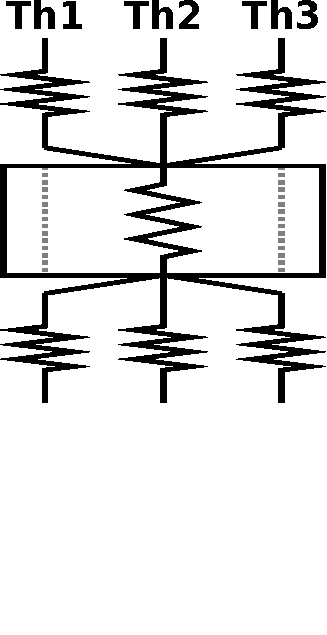
\includegraphics[width=0.26\columnwidth]{figures/mtmpi/th_funneled.pdf}
%     \label{fig:th_mode_funneled}
%   }
%   \hspace{1.0ex}
%   \subfigure[SERIALIZED.] {
%     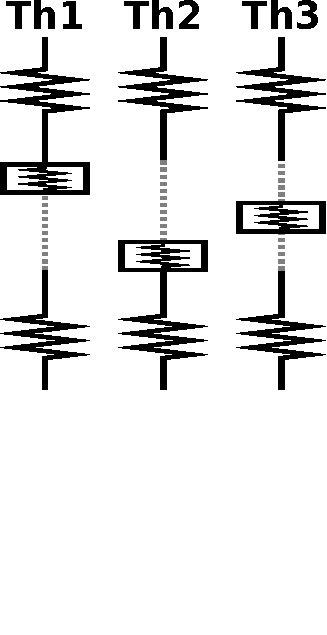
\includegraphics[width=0.26\columnwidth]{figures/mtmpi/th_serialized.pdf}
%     \label{fig:th_mode_serialized}
%   }
%   \hspace{1.0ex}
%   \subfigure[MULTIPLE.] {
%     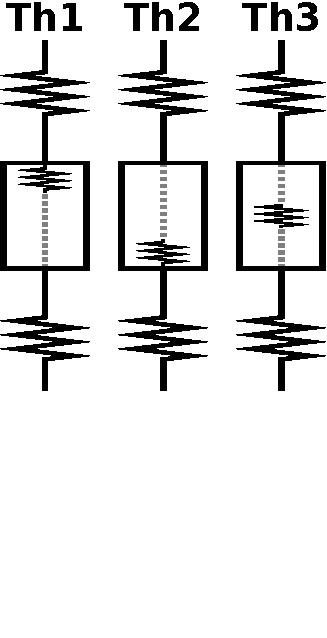
\includegraphics[width=0.26\columnwidth]{figures/mtmpi/th_multiple.pdf}
%     \label{fig:th_mode_mt}
%   }
%   \hspace{0.05\columnwidth}
%   % \vspace{-2.0ex}
%   \caption{Threading modes in MPI.  A line represents a thread; the
%     zigzag part represents an active thread in an OpenMP region; the
%     straight part represents a thread outside an OpenMP region; the
%     dotted part represents an idle thread in an OpenMP region; the
%     boxes represent MPI calls.}
%   \label{fig:th_modes}
%   % \vspace{-3.0ex}
% \end{figure}


\newsavebox\mpiOutsideBox
\begin{lrbox}{\mpiOutsideBox}
\begin{lstlisting}[linewidth=0.45\columnwidth]
#pragma omp parallel
{

  /* user computation */

}

MPI_Function();
\end{lstlisting}
\end{lrbox}

\newsavebox\mpiInsideMasterBox
\begin{lrbox}{\mpiInsideMasterBox}
\begin{lstlisting}[linewidth=0.45\columnwidth]
#pragma omp parallel
{
  /* user computation */
  #pragma omp master
  {
    MPI_Function();
  }
}
\end{lstlisting}
\end{lrbox}

\newsavebox\mpiInsideCriticalBox
\begin{lrbox}{\mpiInsideCriticalBox}
\begin{lstlisting}[linewidth=0.45\columnwidth]
#pragma omp parallel
{
  /* user computation */
  #pragma omp critical
  {
    MPI_Function();
  }
}
\end{lstlisting}
\end{lrbox}

\newsavebox\mpiInsideSingleBox
\begin{lrbox}{\mpiInsideSingleBox}
\begin{lstlisting}[linewidth=0.45\columnwidth]
#pragma omp parallel
{
  /* user computation */
  #pragma omp single
  {
    MPI_Function();
  }
}
\end{lstlisting}
\end{lrbox}

\begin{figure}%[h]
\setlength{\subfigcapskip}{5pt}
\centering
\subfigure[Outside a parallel region] {
  \usebox\mpiOutsideBox
  \label{fig:code_hybrid_outside}
}
\hfill
\subfigure[Inside omp \emp{master} region]{
  \usebox\mpiInsideMasterBox
  \label{fig:code_hybrid_master}
}
\\
\vspace{3.0ex}
\subfigure[Inside omp \emp{critical} region]{
  \usebox\mpiInsideCriticalBox
  \label{fig:code_hybrid_critical}
}
\hfill
\subfigure[Inside omp \emp{single} region] {
  \usebox\mpiInsideSingleBox
  \label{fig:code_hybrid_single}
}
\caption{Different use cases in hybrid MPI+OpenMP.}
\label{fig:code_omp}
\end{figure}

\begin{description}
\item[MPI\_THREAD\_SINGLE] \hfill \\
In this mode, only a single thread exists in every MPI process. This
model is commonly referred to as the MPI-only model, where multiple
MPI processes communicate with each other and no threads are involved.

\item[MPI\_THREAD\_FUNNELED] \hfill \\
In this mode, multiple threads can be created for parallelizing the
computation phases on every MPI process, but only the master thread is
allowed to access MPI stack. In an OpenMP program, this can be implemented
as either making MPI calls outside the OpenMP parallel region or protecting
the MPI calls with OpenMP master regions. Figure~\ref{fig:code_hybrid_outside}
and \ref{fig:code_hybrid_master} demonstrate those implementation
respectively.

\item[MPI\_THREAD\_SERIALIZED] \hfill \\
Similar as the funneled mode, multiple threads can be used to parallelize
the computation in the serialized mode. For the MPI communication phases,
however, any single thread can issue MPI calls at a time. That is, different
threads can concurrently perform the computation, but all of them need to
be synchronized in order to serialize the MPI calls.  In a typical OpenMP
program, this can be implemented by making MPI calls within OpenMP critical
regions or single regions as shown in Figure~\ref{fig:code_hybrid_critical}
and \ref{fig:code_hybrid_single} respectively.

\item[MPI\_THREAD\_MULTIPLE] \hfill \\
The multiple mode is different from the above levels, multiple threads
can concurrently perform both user computation and MPI communication.
The MPI implementation is required to provide appropriate synchronization
among threads (i.e., lock protection and memory barriers) to protect
accesses to shared internal data structures.

\end{description}

%===============================
\subsection{Typical Applications}
%===============================
After a brief overview of the hybrid programming model, we then introduce
two scientific applications that utilize this model.

%------------------------------
\subsubsection{Quantum Monte Carlo Simulation}
%------------------------------
Quantum Monte Carlo (QMC) method is one of the most accurate solution to
provide accurate and reliable approximation for quantum many-body systems.
It helps scientists study the complex electronic structure of realistic
world on large-scale computing systems. The algorithm of QMC method is
mainly designed around two data objects: enormous ``walkers'' to represent
the dynamic status of each particle, and a large but read-only \emp{ensemble}
data that shared among all walkers. The traditional implementation of
QMC method utilizes MPI to distribute the walkers among multiple processes
and simply replicate the ensemble data on each MPI process. However,
such design extremely limits researchers to study larger physical systems
or achieve more accurate simulations since the ensemble data is so large
that always takes Gigabytes memory per core. Especially on modern
mulit- and many-core systems, whose memory capacity per core is actually
reducing, a more efficient design is required.

QMCPACK is an open-source QMC package implemented using hybrid MPI+
threads programming model for massively parallel computing system~\cite{qmcpack}.
It utilizes threads to parallelize the walkers inside every physical node
thus the essential memory restriction can be addressed since the large
\emp{ensemble} data can be shared among threads on every node, and employs MPI
for inter-node communication as demonstrated in Figure~\ref{fig:app-qmcpack}.
This design also benefits from reduced collective communication among
MPI processes that is used for global reduction calculation among walkers,
and from less number of large point-to-point communication between paired
MPI processes for exchanging walker objects in the load balance step.

\begin{figure}[ht]
\centering
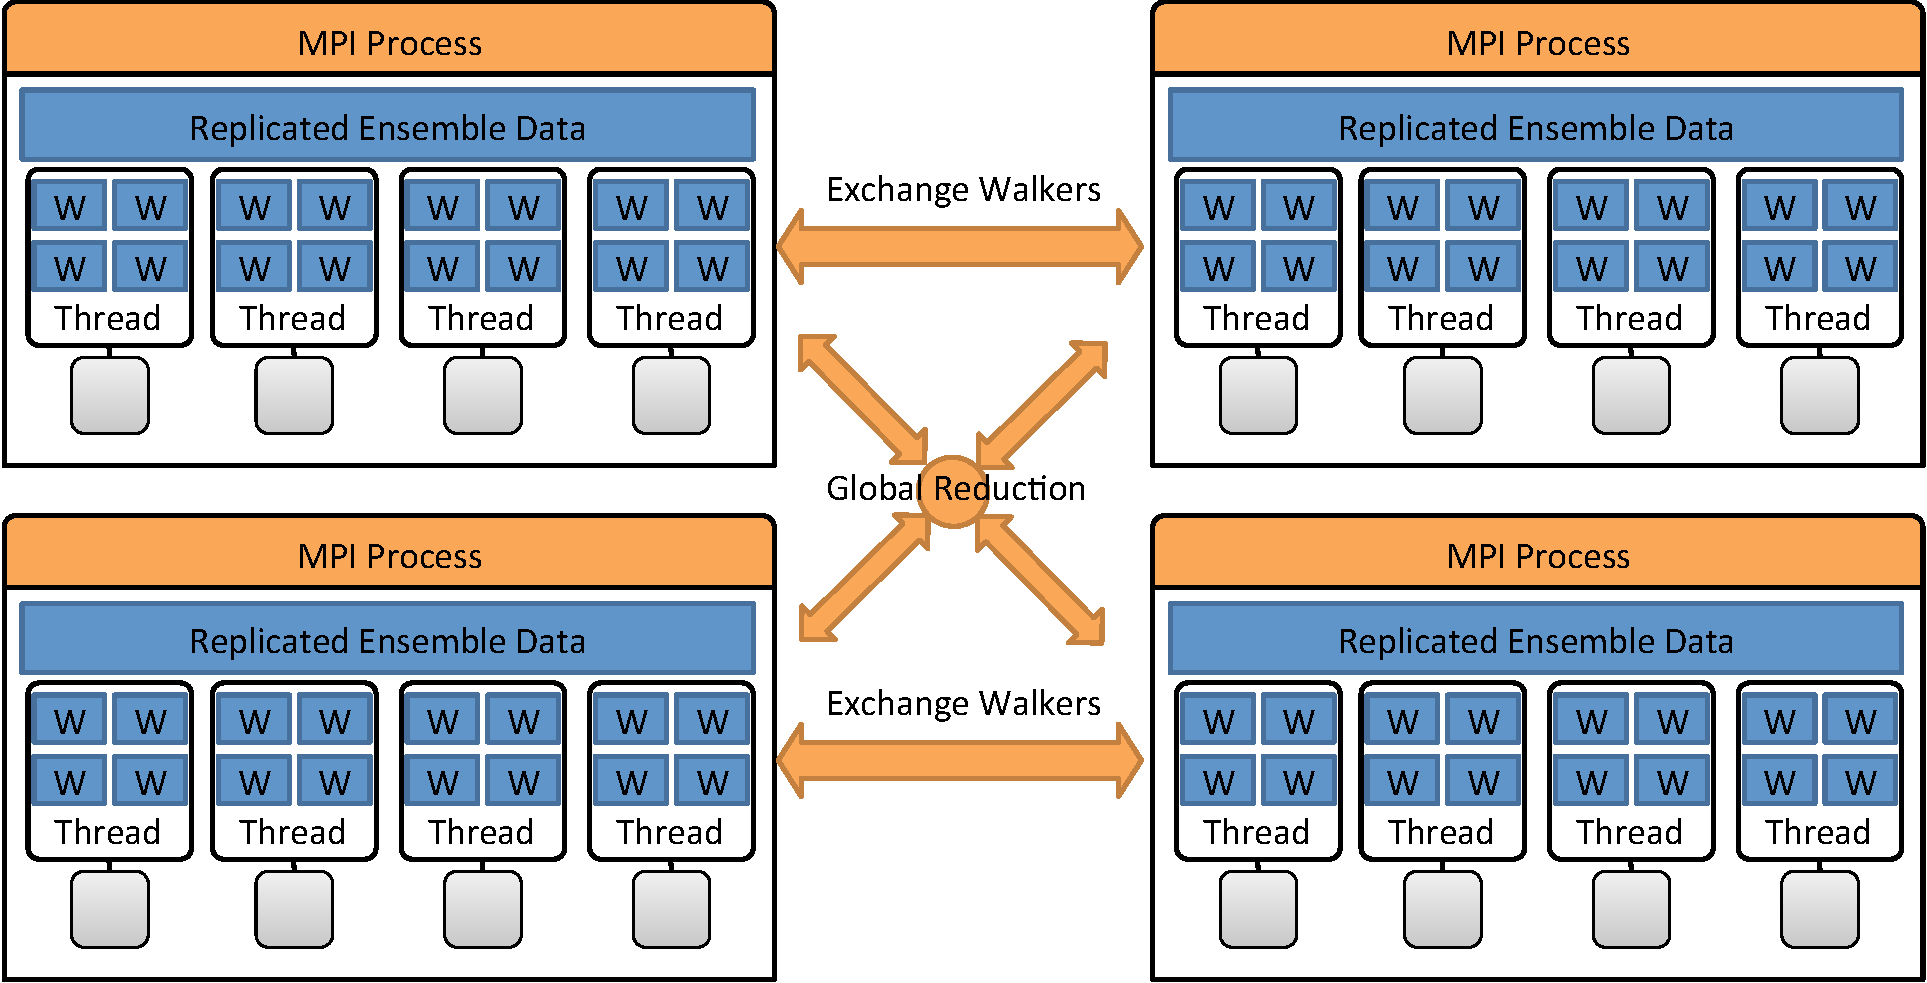
\includegraphics[width=1\textwidth]{figures/background/app-qmcpack.pdf}
\caption{Hybrid Implementation of Quantum Monte Carlo Simulation.}
\label{fig:app-qmcpack}
\end{figure}

%------------------------------
\subsubsection{Computational Fluid Dynamics}
%------------------------------

Nek5000 is an open-source code that widely used in a broad range of
applications such as nuclear reactor cores, ocean modeling and combustion
simulation~\cite{nek5000}. It provides high order, incompressible
Navier-Stokes solver based on the spectral element method. The implementation
of Nek5000 is mainly composed of conjugate gradient (CG) solver with
efficient preconditioners, which is captured in the Nekbone mini-application
with the basic structure and user interface.

The main computational kernel of Nekbone consists of multi-grid matrix-matrix
multiplications. Several researches have looked into the optimization for
such computation pattern on advanced heterogeneous HPC architectures. For
example, Markidis et al.~\cite{nek-openacc} presented an MPI+OpenACC version
of Nek5000 code to highly parallelize the most time-consuming ax3D and
gs\_op subroutines on GPU-accelerated systems. Hart and Ivanov et al.'s papers
~\cite{nek-eva, nek-openmp4} have also contributed the MPI+OpenMP version of
the Nekbone mini-application for accelerating the local computation on
Cray supercomputers.

